\documentclass[a4paper,11pt]{article}
\usepackage{xcolor}
\usepackage{geometry}
\usepackage{hyperref}
\usepackage{graphicx}
\usepackage{float}
\geometry{
a4paper,
total={170mm,257mm},
left=20mm,
top=20mm,
marginparsep=0mm,
}
\setlength\parindent{0pt} % get rid of the stupid indent

\title{DSD Theory Cheatsheet}
\author{Thomas Boxall\\ \texttt{up2108121@myport.ac.uk}}
\date{May 2023}

\usepackage{fancyhdr}
\pagestyle{fancy}
\fancyhead{} % clear all header fields
\renewcommand{\headrulewidth}{0pt} % no line in header area
\fancyfoot{} % clear all footer fields
\renewcommand{\footrulewidth}{0.4pt}
\fancyfoot[C]{\thepage} % page number in centre of the page
\fancyfoot[R]{\footnotesize Thomas Boxall\\ \texttt{up2108121@myport.ac.uk}} % right hand footer has author name on top line and author contact on bottom line
\fancyfoot[L]{\footnotesize DSD Theory Cheatsheet \\ May 2023} % left hand footer has title of document on top line and date on bottom line


\begin{document}

\maketitle
\thispagestyle{fancy}

\section{Data}
\textbf{Data} is facts and statistics collected together for reference or analysis.\\
\textbf{Information} is the result of processing data by adding context and meaning. We should carefully examine the context before drawing information from data.

\section{Database Management System}
The \textit{DataBase Management System} (DBMS) is the core of the database system. All communication to the database goes through DBMS. \\
DBMS controls users, access to data \& schema and provides an view of operations. DBMS removes risk of inconsistent data \& improves the ease which security can be controlled with.\\
Two different languages are used to interface with a database. \textit{Data Definition Language} (DDL) defines the structure of the database. \textit{Data Manipulation Language} (DML) is used to manipulate the data. 

\section{Entities \& where we keep them}
\textbf{Entity} a `thing' about which data is stored (often will be nouns). These should be singular, not plural.\\
\textbf{Attribute} a quality of an entity (eg id number, name, etc)\\
\textbf{Table} A 2D representation of entities. (AKA relation table or relation).\\
\textbf{Record} a row of data in a table. (AKA tuple or row).\\
\textbf{Relationship} is how two tables are related to each other, they are represented in relations. \\
When designing a database we have to think about the entities we will store, what data about them we need, and what form this data will take.

\subsection{Entity Relationship Diagrams}
\textbf{ERD} a diagram showing how entities \& attributes are related. They are built from business rules (\textit{statements that define how companies do things}). Entities are joined up using `Crows Foot Notation'.
\begin{figure}[H]
    \centering
    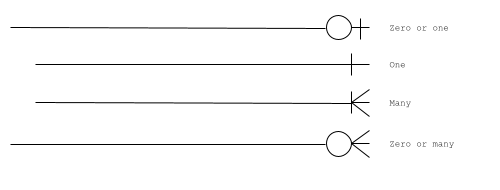
\includegraphics[width=0.9\textwidth]{../assets/relationship-links.png}
    \caption{Crow's foot notation}
\end{figure}

\section{Keys}
\textbf{Primary Key} an attribute (or combination of attributes) which uniquely identifies a record. Every table must have one.\\
\textbf{Composite Key} a combination of attributes (each called simple keys) that act as a primary key in a table.\\
\textbf{Foreign Key} an attribute (or combination of attributes) which is a primary key in another table.\\
\textbf{Alternate Key} gives an alternate access path to data that is not via the primary key. This is \textit{bad} and if correctly normalised, this shouldn't exist. 

\section{Attributes}
\textbf{Constraint} a rule that protects your data or enforces certain behaviour.\\
All the different bits of data we store about an entity will all be different attributes. The data we store has to be GDPR compliant (must be: adequate, relevant and limited to what is necessary).
\subsection{Data Types}
\textit{see \href{https://thomasboxall.github.io/uni-notes/01-FIRST-YEAR/M30232-databaseSystemsDevelopment/M30232.pdf}{my notes} for more details on each data type.}\\
\textbf{Numerical} smallint, integer, bigint, decimal, real, double, serial, bigserial\\
\textbf{Alphanumeric} text, char, varchar\\
\textbf{Date \& time} timestamp without timezone, timestamp with timezone, date, time without timezone, time with timezone.

\section{Normalisation}


\end{document}